\documentclass{article}
\usepackage[utf8]{inputenc}
\usepackage[T5]{fontenc}
\usepackage{graphicx}
\usepackage[margin=2cm]{geometry}
\title{Report 8: RGB--HSV Conversion}
\author{Nguyễn Thanh Hùng -- 2540056}
\date{}

\begin{document}
\maketitle

\section{Implementation}
I converted interleaved RGB pixels into separate H, S and V arrays, then converted these arrays back to RGB. Each thread processes one pixel using a $16\times16$ block. H is stored in degrees; S and V are in $[0,1]$. I compared HSV with Matplotlib and the reconstructed RGB with the input.

I ran the notebook on Google Colab with a Tesla T4 and a $256\times256$ sample image.
GPU timings use \texttt{time.time()} after warm-up and synchronization, averaged over three runs; allocation and image transfers are excluded. Where measured, CPU time is one run; speedup is relative to that Python CPU implementation.

\section{Results}
\begin{center}
\begin{tabular}{lr}
\hline
Operation & GPU (ms) \\
\hline
RGB to HSV & 0.1892 \\
HSV to RGB & 0.1217 \\
\hline
\end{tabular}
\end{center}
Maximum normalized hue error: $7.09\times10^{-8}$. Maximum RGB reconstruction error: 0.
\begin{center}
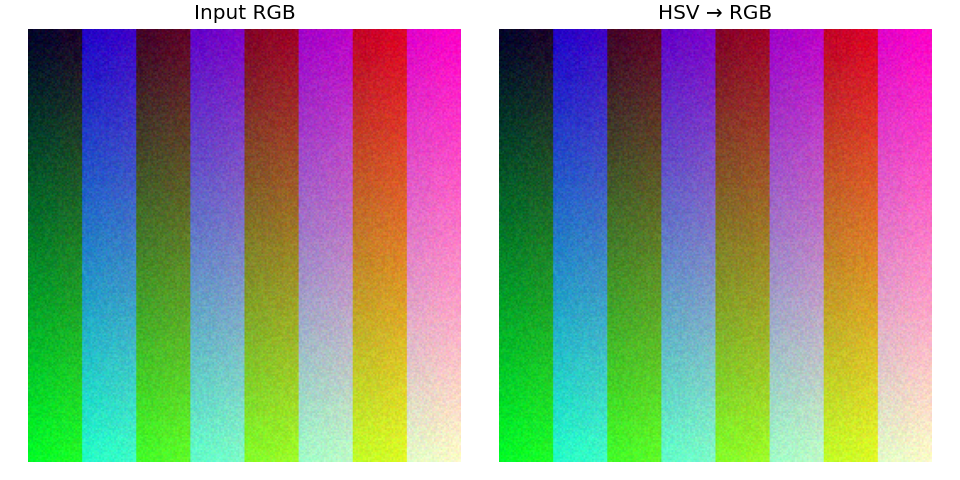
\includegraphics[width=.85\linewidth,height=.19\textheight,keepaspectratio]{figures/images.png}
\end{center}
\begin{center}
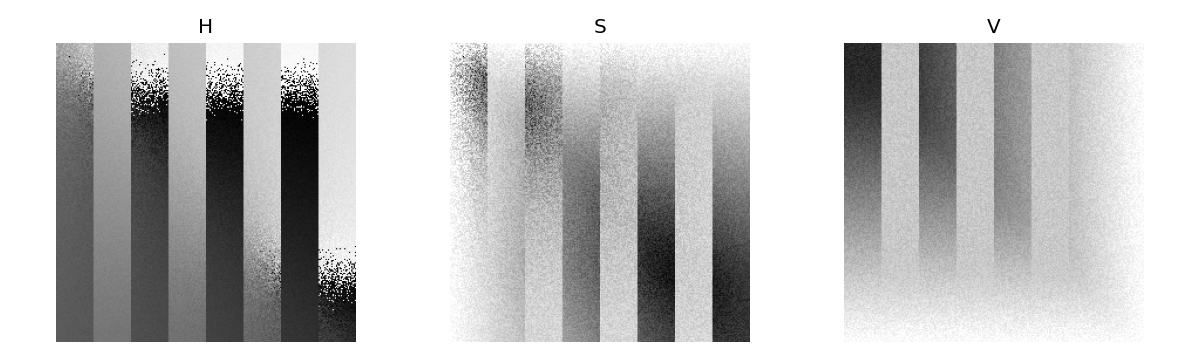
\includegraphics[width=.85\linewidth,height=.17\textheight,keepaspectratio]{figures/hsv.png}
\end{center}

\section{Discussion}
The reconstructed RGB image exactly matched the input in this run. The separate H, S and V arrays allow later kernels to read one channel independently.

\end{document}
